% ============================================================================
% AD7031 Week 6 -- LECTURE NOTE
%
% Section 1 -- the two classical results named at the end of the course
% folder's handwritten "OUU Lecture 3", p.2 (titles only there): LLN and CLT
% stated as in G. Hanasusanto, "Optimization Under Uncertainty" (Fall 2016),
% Section 1.2; coin-toss example and figures added.
%
% Sections 2-5 -- straight conversion of the handwritten "OUU Lecture 3" (5 pp.):
%   p.1   duality theory -- (P), (D), the sup-trick, weak/strong duality, Slater
%   p.2   LP example -- primal LP to dual LP, LP strong duality
%   p.3   conic programming -- cone, proper cone, generic conic program, LP
%   p.4   SDP, second-order cone, dual cone, self-dual cones
%   p.5   primal / dual conic program
% Same house style as OUU_week02_note.tex; self-contained -- no \input.
% ============================================================================
\documentclass[10pt]{article}

\usepackage[a4paper, margin=1.9cm]{geometry}
\usepackage{amsmath, amssymb}
\usepackage[dvipsnames]{xcolor}
\usepackage{graphicx}
\usepackage{array}
\usepackage{colortbl}
\usepackage{tikz}
\usepackage[hidelinks]{hyperref}

\definecolor{ruleink}{RGB}{18, 68, 140}
\definecolor{demoink}{RGB}{140, 82, 20}
\definecolor{keyink}{RGB}{20, 90, 20}
\definecolor{watchink}{RGB}{86, 60, 140}
\definecolor{punchink}{RGB}{170, 30, 60}
\definecolor{lineA}{RGB}{44, 110, 176}
\definecolor{lineB}{RGB}{168, 96, 32}
\definecolor{lineC}{RGB}{78, 62, 140}

% ---- the pens used in the handwritten original ----------------------------
\definecolor{redink}{RGB}{198, 38, 38}
\definecolor{purpink}{RGB}{132, 58, 176}
\definecolor{grnink}{RGB}{22, 118, 62}
\definecolor{magink}{RGB}{214, 30, 158}
\definecolor{boxink}{RGB}{232, 150, 42}
\definecolor{sandink}{RGB}{250, 206, 142}
\definecolor{hlyel}{RGB}{255, 244, 130}

\setlength{\parindent}{0pt}
\pagestyle{empty}

% tighter spacing around centered displays
\AtBeginDocument{%
  \abovedisplayskip=7pt plus 2pt
  \belowdisplayskip=7pt plus 2pt
  \abovedisplayshortskip=4pt
  \belowdisplayshortskip=4pt}

% ---- one section -----------------------------------------------------------
\newcommand{\beat}[2]{%   number, title
  \par\bigskip\vspace{4pt}
  {\color{ruleink}\rule{\textwidth}{1pt}}\par\nobreak\vspace{4pt}
  {\large\bfseries #1.\; #2}\par\nobreak\vspace{6pt}}

% ---- board content ---------------------------------------------------------
\newenvironment{board}{%
  \par\vspace{4pt}
  \begingroup\leftskip=1.3em\relax\parskip=2pt\relax}{%
  \par\endgroup\vspace{4pt}}

% ---- hanging bullet (wrapped lines stay indented) --------------------------
\newcommand{\bul}{\hangindent=2.6em\hangafter=1\hspace{1.2em}\textbullet\ \ignorespaces}

% ---- cone order and highlighter -------------------------------------------
\newcommand{\coneleq}{\mathrel{\preceq_{\scriptscriptstyle C}}}
\newcommand{\hl}[1]{\colorbox{hlyel}{$#1$}}

\begin{document}

{\Large\bfseries Week 6 --- LLN and CLT, Duality Theory, Conic Programming}\\[2pt]
{\small AD7031 Optimization Under Uncertainty \quad\textbullet\quad Instructor: Prof.\ H.\ Park \quad\textbullet\quad Oct 3, 2026}

% ---------------------------------------------------------------- 1
\beat{1}{Two classical results in probability theory}
\begin{board}
$\tilde\xi_1, \tilde\xi_2, \tilde\xi_3, \dots$ \ : \ an infinite sequence of \textbf{independent and identically
distributed (i.i.d.)} random variables,
\vspace{3pt}

\quad each with expected value $\mu$ \ and variance $\sigma^2$
\vspace{16pt}

\textbf{1) Law of large numbers} \quad (strong law, SLLN)
\vspace{4pt}

\begin{center}
$\displaystyle \mathbb{P}\Big( \lim_{S \to \infty}\ \frac{1}{S} \sum_{i \in [S]} \tilde\xi_i \;=\; \mu \Big) \;=\; 1$
\end{center}
\vspace{2pt}

\hspace{5.0cm}{\color{redink}sample average \ $\longrightarrow$ \ expected value}
\vspace{14pt}

\textbf{Example} \quad toss a fair coin: \quad
$\tilde\xi_i = \begin{cases} 1 & \text{if toss } i \text{ is head} \\ 0 & \text{if toss } i \text{ is tail} \end{cases}$
\vspace{6pt}

\quad $\mu = \tfrac12$, \qquad $\sigma^2 = \mathbb{E}[\tilde\xi_i^2] - \mu^2 = \tfrac12 - \tfrac14 = \tfrac14$
\vspace{4pt}

\quad $\dfrac{1}{S} \displaystyle\sum_{i \in [S]} \tilde\xi_i$ \ = \ fraction of heads in the first $S$ tosses
\vspace{8pt}

\begin{center}
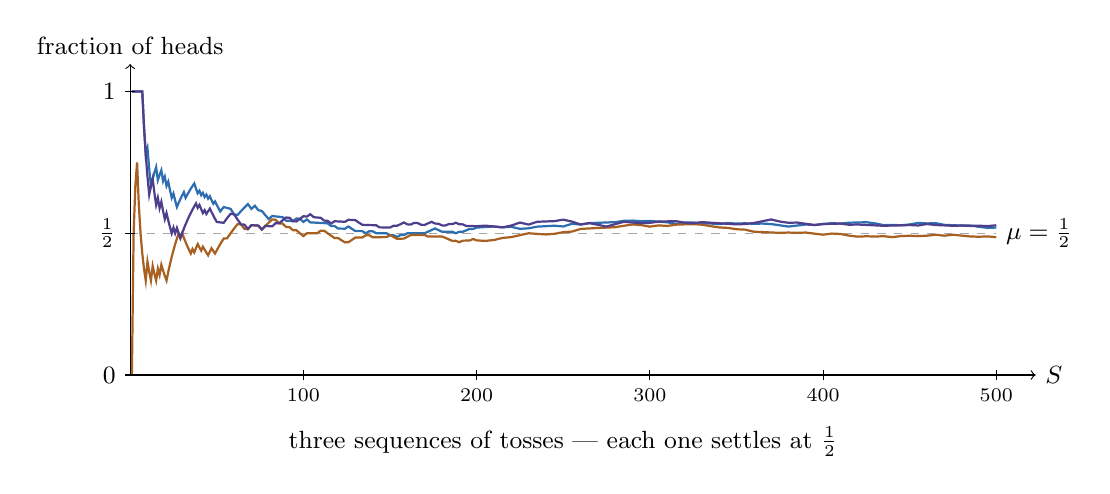
\begin{tikzpicture}[font=\small]
  \draw[dashed, gray!70] (0,1.8) -- (11,1.8) node[right, black] {$\mu = \tfrac12$};
  \draw[lineA, thick] plot coordinates {(0.022,3.600) (0.044,3.600) (0.066,3.600) (0.088,3.600) (0.110,3.600) (0.132,3.600) (0.154,3.600) (0.176,3.150) (0.198,2.800) (0.220,2.880) (0.242,2.618) (0.264,2.400) (0.286,2.492) (0.308,2.571) (0.330,2.640) (0.352,2.475) (0.374,2.541) (0.396,2.600) (0.418,2.463) (0.440,2.520) (0.462,2.400) (0.484,2.455) (0.506,2.348) (0.528,2.250) (0.550,2.304) (0.572,2.215) (0.594,2.133) (0.616,2.186) (0.638,2.234) (0.660,2.280) (0.682,2.323) (0.704,2.250) (0.726,2.291) (0.748,2.329) (0.770,2.366) (0.792,2.400) (0.814,2.432) (0.836,2.368) (0.858,2.308) (0.880,2.340) (0.902,2.283) (0.924,2.314) (0.946,2.260) (0.968,2.291) (0.990,2.240) (1.012,2.270) (1.034,2.221) (1.056,2.175) (1.078,2.204) (1.100,2.160) (1.144,2.077) (1.188,2.133) (1.232,2.121) (1.276,2.110) (1.320,2.040) (1.364,2.032) (1.408,2.081) (1.452,2.127) (1.496,2.171) (1.540,2.109) (1.584,2.150) (1.628,2.092) (1.672,2.084) (1.716,2.031) (1.760,1.980) (1.804,2.020) (1.848,2.014) (1.892,2.009) (1.936,2.005) (1.980,1.960) (2.024,1.957) (2.068,1.953) (2.112,1.988) (2.156,1.984) (2.200,1.944) (2.244,1.976) (2.288,1.938) (2.332,1.936) (2.376,1.933) (2.420,1.931) (2.464,1.929) (2.508,1.926) (2.552,1.893) (2.596,1.892) (2.640,1.860) (2.684,1.859) (2.728,1.858) (2.772,1.886) (2.816,1.856) (2.860,1.828) (2.904,1.827) (2.948,1.827) (2.992,1.800) (3.036,1.826) (3.080,1.826) (3.124,1.800) (3.168,1.800) (3.212,1.800) (3.256,1.800) (3.300,1.776) (3.344,1.776) (3.388,1.753) (3.432,1.777) (3.476,1.777) (3.520,1.800) (3.564,1.800) (3.608,1.800) (3.652,1.800) (3.696,1.800) (3.740,1.800) (3.784,1.821) (3.828,1.841) (3.872,1.861) (3.916,1.840) (3.960,1.820) (4.004,1.820) (4.048,1.820) (4.092,1.819) (4.136,1.800) (4.180,1.819) (4.224,1.819) (4.268,1.837) (4.312,1.855) (4.356,1.855) (4.400,1.872) (4.510,1.879) (4.620,1.886) (4.730,1.875) (4.840,1.882) (4.950,1.856) (5.060,1.863) (5.170,1.884) (5.280,1.890) (5.390,1.896) (5.500,1.886) (5.610,1.920) (5.720,1.911) (5.830,1.929) (5.940,1.933) (6.050,1.937) (6.160,1.941) (6.270,1.958) (6.380,1.961) (6.490,1.953) (6.600,1.956) (6.710,1.948) (6.820,1.939) (6.930,1.920) (7.040,1.935) (7.150,1.938) (7.260,1.920) (7.370,1.924) (7.480,1.916) (7.590,1.930) (7.700,1.923) (7.810,1.927) (7.920,1.920) (8.030,1.923) (8.140,1.917) (8.250,1.901) (8.360,1.885) (8.470,1.898) (8.580,1.911) (8.690,1.905) (8.800,1.917) (8.910,1.929) (9.020,1.923) (9.130,1.934) (9.240,1.937) (9.350,1.940) (9.460,1.926) (9.570,1.903) (9.680,1.906) (9.790,1.901) (9.900,1.912) (10.010,1.931) (10.120,1.925) (10.230,1.928) (10.340,1.907) (10.450,1.902) (10.560,1.898) (10.670,1.900) (10.780,1.881) (10.890,1.869) (11.000,1.872)};
  \draw[lineB, thick] plot coordinates {(0.022,0.000) (0.044,1.800) (0.066,2.400) (0.088,2.700) (0.110,2.160) (0.132,1.800) (0.154,1.543) (0.176,1.350) (0.198,1.200) (0.220,1.440) (0.242,1.309) (0.264,1.200) (0.286,1.385) (0.308,1.286) (0.330,1.200) (0.352,1.350) (0.374,1.271) (0.396,1.400) (0.418,1.326) (0.440,1.260) (0.462,1.200) (0.484,1.309) (0.506,1.409) (0.528,1.500) (0.550,1.584) (0.572,1.662) (0.594,1.733) (0.616,1.800) (0.638,1.738) (0.660,1.800) (0.682,1.742) (0.704,1.688) (0.726,1.636) (0.748,1.588) (0.770,1.543) (0.792,1.600) (0.814,1.557) (0.836,1.611) (0.858,1.662) (0.880,1.620) (0.902,1.580) (0.924,1.629) (0.946,1.591) (0.968,1.555) (0.990,1.520) (1.012,1.565) (1.034,1.609) (1.056,1.575) (1.078,1.543) (1.100,1.584) (1.144,1.662) (1.188,1.733) (1.232,1.736) (1.276,1.800) (1.320,1.860) (1.364,1.916) (1.408,1.913) (1.452,1.855) (1.496,1.853) (1.540,1.903) (1.584,1.900) (1.628,1.897) (1.672,1.847) (1.716,1.892) (1.760,1.935) (1.804,1.976) (1.848,1.971) (1.892,1.926) (1.936,1.923) (1.980,1.880) (2.024,1.878) (2.068,1.838) (2.112,1.837) (2.156,1.800) (2.200,1.764) (2.244,1.800) (2.288,1.800) (2.332,1.800) (2.376,1.800) (2.420,1.833) (2.464,1.832) (2.508,1.800) (2.552,1.769) (2.596,1.739) (2.640,1.740) (2.684,1.711) (2.728,1.684) (2.772,1.686) (2.816,1.716) (2.860,1.745) (2.904,1.745) (2.948,1.746) (2.992,1.774) (3.036,1.774) (3.080,1.749) (3.124,1.749) (3.168,1.750) (3.212,1.751) (3.256,1.751) (3.300,1.776) (3.344,1.753) (3.388,1.730) (3.432,1.731) (3.476,1.732) (3.520,1.755) (3.564,1.778) (3.608,1.778) (3.652,1.778) (3.696,1.779) (3.740,1.779) (3.784,1.758) (3.828,1.759) (3.872,1.759) (3.916,1.760) (3.960,1.760) (4.004,1.741) (4.048,1.722) (4.092,1.703) (4.136,1.704) (4.180,1.686) (4.224,1.706) (4.268,1.707) (4.312,1.708) (4.356,1.727) (4.400,1.710) (4.510,1.703) (4.620,1.714) (4.730,1.741) (4.840,1.751) (4.950,1.776) (5.060,1.800) (5.170,1.792) (5.280,1.785) (5.390,1.793) (5.500,1.814) (5.610,1.821) (5.720,1.855) (5.830,1.861) (5.940,1.867) (6.050,1.872) (6.160,1.877) (6.270,1.895) (6.380,1.912) (6.490,1.904) (6.600,1.884) (6.710,1.900) (6.820,1.893) (6.930,1.909) (7.040,1.913) (7.150,1.916) (7.260,1.909) (7.370,1.891) (7.480,1.874) (7.590,1.868) (7.700,1.851) (7.810,1.846) (7.920,1.820) (8.030,1.815) (8.140,1.810) (8.250,1.805) (8.360,1.809) (8.470,1.805) (8.580,1.809) (8.690,1.795) (8.800,1.782) (8.910,1.796) (9.020,1.791) (9.130,1.770) (9.240,1.757) (9.350,1.762) (9.460,1.758) (9.570,1.763) (9.680,1.751) (9.790,1.764) (9.900,1.768) (10.010,1.764) (10.120,1.769) (10.230,1.781) (10.340,1.769) (10.450,1.781) (10.560,1.770) (10.670,1.759) (10.780,1.756) (10.890,1.760) (11.000,1.750)};
  \draw[lineC, thick] plot coordinates {(0.022,3.600) (0.044,3.600) (0.066,3.600) (0.088,3.600) (0.110,3.600) (0.132,3.600) (0.154,3.600) (0.176,3.150) (0.198,2.800) (0.220,2.520) (0.242,2.291) (0.264,2.400) (0.286,2.492) (0.308,2.314) (0.330,2.160) (0.352,2.250) (0.374,2.118) (0.396,2.200) (0.418,2.084) (0.440,1.980) (0.462,2.057) (0.484,1.964) (0.506,1.878) (0.528,1.800) (0.550,1.872) (0.572,1.800) (0.594,1.867) (0.616,1.800) (0.638,1.738) (0.660,1.800) (0.682,1.858) (0.704,1.913) (0.726,1.964) (0.748,2.012) (0.770,2.057) (0.792,2.100) (0.814,2.141) (0.836,2.179) (0.858,2.123) (0.880,2.160) (0.902,2.107) (0.924,2.057) (0.946,2.093) (0.968,2.045) (0.990,2.080) (1.012,2.113) (1.034,2.068) (1.056,2.025) (1.078,1.984) (1.100,1.944) (1.144,1.938) (1.188,1.933) (1.232,1.993) (1.276,2.048) (1.320,2.040) (1.364,1.974) (1.408,1.913) (1.452,1.909) (1.496,1.853) (1.540,1.903) (1.584,1.900) (1.628,1.897) (1.672,1.847) (1.716,1.892) (1.760,1.890) (1.804,1.888) (1.848,1.929) (1.892,1.926) (1.936,1.964) (1.980,2.000) (2.024,1.996) (2.068,1.953) (2.112,1.950) (2.156,1.984) (2.200,2.016) (2.244,2.012) (2.288,2.042) (2.332,2.004) (2.376,2.000) (2.420,1.996) (2.464,1.961) (2.508,1.958) (2.552,1.924) (2.596,1.953) (2.640,1.950) (2.684,1.948) (2.728,1.945) (2.772,1.971) (2.816,1.969) (2.860,1.966) (2.904,1.936) (2.948,1.907) (2.992,1.906) (3.036,1.904) (3.080,1.903) (3.124,1.901) (3.168,1.875) (3.212,1.874) (3.256,1.873) (3.300,1.872) (3.344,1.895) (3.388,1.894) (3.432,1.915) (3.476,1.937) (3.520,1.913) (3.564,1.911) (3.608,1.932) (3.652,1.930) (3.696,1.907) (3.740,1.906) (3.784,1.926) (3.828,1.945) (3.872,1.923) (3.916,1.921) (3.960,1.900) (4.004,1.899) (4.048,1.917) (4.092,1.916) (4.136,1.934) (4.180,1.914) (4.224,1.913) (4.268,1.893) (4.312,1.892) (4.356,1.891) (4.400,1.890) (4.510,1.897) (4.620,1.886) (4.730,1.875) (4.840,1.898) (4.950,1.936) (5.060,1.910) (5.170,1.946) (5.280,1.950) (5.390,1.954) (5.500,1.973) (5.610,1.948) (5.720,1.911) (5.830,1.929) (5.940,1.907) (6.050,1.885) (6.160,1.916) (6.270,1.945) (6.380,1.937) (6.490,1.928) (6.600,1.932) (6.710,1.948) (6.820,1.951) (6.930,1.954) (7.040,1.935) (7.150,1.927) (7.260,1.942) (7.370,1.934) (7.480,1.927) (7.590,1.920) (7.700,1.913) (7.810,1.917) (7.920,1.930) (8.030,1.953) (8.140,1.975) (8.250,1.949) (8.360,1.933) (8.470,1.936) (8.580,1.920) (8.690,1.905) (8.800,1.917) (8.910,1.920) (9.020,1.923) (9.130,1.908) (9.240,1.911) (9.350,1.906) (9.460,1.900) (9.570,1.895) (9.680,1.898) (9.790,1.901) (9.900,1.904) (10.010,1.899) (10.120,1.917) (10.230,1.905) (10.340,1.900) (10.450,1.895) (10.560,1.898) (10.670,1.893) (10.780,1.896) (10.890,1.891) (11.000,1.901)};
  \draw[->] (0,0) -- (11.5,0) node[right] {$S$};
  \draw[->] (0,0) -- (0,3.95) node[above] {fraction of heads};
  \foreach \i in {100,200,300,400,500}
    { \draw (\i/500*11,0.06) -- (\i/500*11,-0.06) node[below] {\scriptsize $\i$}; }
  \foreach \v/\lab in {0/0, 1.8/\tfrac12, 3.6/1}
    { \draw (0.06,\v) -- (-0.06,\v) node[left] {$\lab$}; }
  \node at (5.5,-0.85) {three sequences of tosses --- each one settles at $\tfrac12$};
\end{tikzpicture}
\end{center}
\newpage

\textbf{2) Central limit theorem} \quad (CLT)
\vspace{6pt}

\quad $\tilde\chi_S = \displaystyle\sum_{i \in [S]} \tilde\xi_i$ \qquad
{\color{redink}$\mathbb{E}[\tilde\chi_S] = S\mu$, \quad $\mathrm{Var}(\tilde\chi_S) = S\sigma^2$}
\vspace{10pt}

\quad for large $S$, \ the random variable \ $\dfrac{\tilde\chi_S - S\mu}{\sigma\sqrt{S}}$ \ is approximately \textbf{standard normal}:
\vspace{6pt}

\begin{center}
$\displaystyle \mathbb{P}\Big( \frac{\tilde\chi_S - S\mu}{\sigma\sqrt{S}} \le r \Big) \ \longrightarrow\ \mathbb{P}(\tilde\zeta \le r)
\quad \text{as } S \to \infty \quad \forall r \in \mathbb{R}, \qquad \tilde\zeta \sim \mathcal{N}(0,1)$
\end{center}
\vspace{2pt}

\hspace{5.0cm}{\color{redink}whatever the distribution of $\tilde\xi_i$}
\vspace{10pt}

\quad divide by $S$: \qquad $\dfrac{1}{S}\tilde\chi_S \ \approx\ \mathcal{N}\Big(\mu, \ \dfrac{\sigma^2}{S}\Big)$,
\qquad std dev \ $\dfrac{\sigma}{\sqrt{S}}$
\vspace{14pt}

\textbf{Example} \quad same coin: \quad $\tilde\chi_S$ = number of heads in $S$ tosses, \qquad
$\tfrac{1}{S}\tilde\chi_S$ = fraction of heads
\vspace{8pt}

\begin{center}
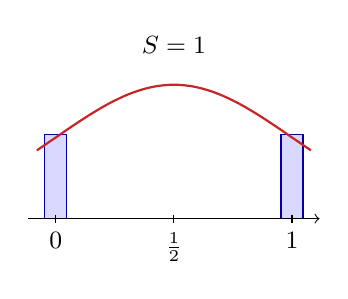
\begin{tikzpicture}[font=\small]
  \draw[fill=blue!15, draw=blue!65!black] (-0.140,0) rectangle (0.140,1.065);
  \draw[fill=blue!15, draw=blue!65!black] (2.860,0) rectangle (3.140,1.065);
  \draw[redink, thick] plot[smooth] coordinates {(-0.240,0.867) (-0.201,0.894) (-0.162,0.920) (-0.123,0.947) (-0.084,0.974) (-0.044,1.001) (-0.005,1.027) (0.034,1.054) (0.073,1.081) (0.112,1.108) (0.151,1.135) (0.190,1.161) (0.229,1.187) (0.268,1.213) (0.307,1.239) (0.347,1.265) (0.386,1.290) (0.425,1.315) (0.464,1.339) (0.503,1.363) (0.542,1.386) (0.581,1.409) (0.620,1.431) (0.659,1.453) (0.698,1.474) (0.738,1.494) (0.777,1.513) (0.816,1.532) (0.855,1.550) (0.894,1.567) (0.933,1.583) (0.972,1.598) (1.011,1.612) (1.050,1.625) (1.089,1.637) (1.129,1.649) (1.168,1.659) (1.207,1.668) (1.246,1.676) (1.285,1.683) (1.324,1.688) (1.363,1.693) (1.402,1.696) (1.441,1.699) (1.480,1.700) (1.520,1.700) (1.559,1.699) (1.598,1.696) (1.637,1.693) (1.676,1.688) (1.715,1.683) (1.754,1.676) (1.793,1.668) (1.832,1.659) (1.871,1.649) (1.911,1.637) (1.950,1.625) (1.989,1.612) (2.028,1.598) (2.067,1.583) (2.106,1.567) (2.145,1.550) (2.184,1.532) (2.223,1.513) (2.262,1.494) (2.302,1.474) (2.341,1.453) (2.380,1.431) (2.419,1.409) (2.458,1.386) (2.497,1.363) (2.536,1.339) (2.575,1.315) (2.614,1.290) (2.653,1.265) (2.693,1.239) (2.732,1.213) (2.771,1.187) (2.810,1.161) (2.849,1.135) (2.888,1.108) (2.927,1.081) (2.966,1.054) (3.005,1.027) (3.044,1.001) (3.084,0.974) (3.123,0.947) (3.162,0.920) (3.201,0.894) (3.240,0.867)};
  \draw[->] (-0.35,0) -- (3.35,0);
  \foreach \v/\lab in {0/0, 1.5/\tfrac12, 3.0/1}
    { \draw (\v,0.05) -- (\v,-0.05) node[below] {$\lab$}; }
  \node at (1.5,2.2) {$S = 1$};
\end{tikzpicture}
\hspace{3mm}
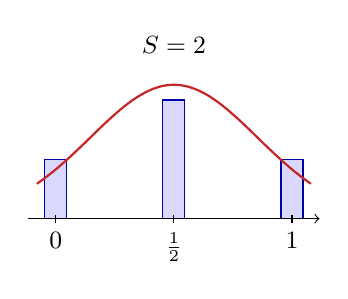
\begin{tikzpicture}[font=\small]
  \draw[fill=blue!15, draw=blue!65!black] (-0.140,0) rectangle (0.140,0.753);
  \draw[fill=blue!15, draw=blue!65!black] (1.360,0) rectangle (1.640,1.507);
  \draw[fill=blue!15, draw=blue!65!black] (2.860,0) rectangle (3.140,0.753);
  \draw[redink, thick] plot[smooth] coordinates {(-0.240,0.443) (-0.201,0.470) (-0.162,0.498) (-0.123,0.527) (-0.084,0.558) (-0.044,0.589) (-0.005,0.621) (0.034,0.654) (0.073,0.688) (0.112,0.722) (0.151,0.757) (0.190,0.793) (0.229,0.829) (0.268,0.866) (0.307,0.903) (0.347,0.941) (0.386,0.979) (0.425,1.017) (0.464,1.055) (0.503,1.093) (0.542,1.131) (0.581,1.168) (0.620,1.205) (0.659,1.242) (0.698,1.278) (0.738,1.313) (0.777,1.347) (0.816,1.381) (0.855,1.413) (0.894,1.444) (0.933,1.474) (0.972,1.502) (1.011,1.529) (1.050,1.554) (1.089,1.577) (1.129,1.599) (1.168,1.619) (1.207,1.636) (1.246,1.652) (1.285,1.665) (1.324,1.677) (1.363,1.686) (1.402,1.693) (1.441,1.697) (1.480,1.700) (1.520,1.700) (1.559,1.697) (1.598,1.693) (1.637,1.686) (1.676,1.677) (1.715,1.665) (1.754,1.652) (1.793,1.636) (1.832,1.619) (1.871,1.599) (1.911,1.577) (1.950,1.554) (1.989,1.529) (2.028,1.502) (2.067,1.474) (2.106,1.444) (2.145,1.413) (2.184,1.381) (2.223,1.347) (2.262,1.313) (2.302,1.278) (2.341,1.242) (2.380,1.205) (2.419,1.168) (2.458,1.131) (2.497,1.093) (2.536,1.055) (2.575,1.017) (2.614,0.979) (2.653,0.941) (2.693,0.903) (2.732,0.866) (2.771,0.829) (2.810,0.793) (2.849,0.757) (2.888,0.722) (2.927,0.688) (2.966,0.654) (3.005,0.621) (3.044,0.589) (3.084,0.558) (3.123,0.527) (3.162,0.498) (3.201,0.470) (3.240,0.443)};
  \draw[->] (-0.35,0) -- (3.35,0);
  \foreach \v/\lab in {0/0, 1.5/\tfrac12, 3.0/1}
    { \draw (\v,0.05) -- (\v,-0.05) node[below] {$\lab$}; }
  \node at (1.5,2.2) {$S = 2$};
\end{tikzpicture}
\hspace{3mm}
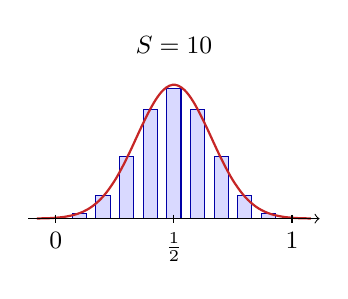
\begin{tikzpicture}[font=\small]
  \draw[fill=blue!15, draw=blue!65!black] (-0.090,0) rectangle (0.090,0.007);
  \draw[fill=blue!15, draw=blue!65!black] (0.210,0) rectangle (0.390,0.066);
  \draw[fill=blue!15, draw=blue!65!black] (0.510,0) rectangle (0.690,0.296);
  \draw[fill=blue!15, draw=blue!65!black] (0.810,0) rectangle (0.990,0.790);
  \draw[fill=blue!15, draw=blue!65!black] (1.110,0) rectangle (1.290,1.382);
  \draw[fill=blue!15, draw=blue!65!black] (1.410,0) rectangle (1.590,1.658);
  \draw[fill=blue!15, draw=blue!65!black] (1.710,0) rectangle (1.890,1.382);
  \draw[fill=blue!15, draw=blue!65!black] (2.010,0) rectangle (2.190,0.790);
  \draw[fill=blue!15, draw=blue!65!black] (2.310,0) rectangle (2.490,0.296);
  \draw[fill=blue!15, draw=blue!65!black] (2.610,0) rectangle (2.790,0.066);
  \draw[fill=blue!15, draw=blue!65!black] (2.910,0) rectangle (3.090,0.007);
  \draw[redink, thick] plot[smooth] coordinates {(-0.240,0.002) (-0.201,0.003) (-0.162,0.004) (-0.123,0.005) (-0.084,0.006) (-0.044,0.008) (-0.005,0.011) (0.034,0.014) (0.073,0.018) (0.112,0.023) (0.151,0.030) (0.190,0.038) (0.229,0.047) (0.268,0.058) (0.307,0.072) (0.347,0.088) (0.386,0.108) (0.425,0.130) (0.464,0.156) (0.503,0.187) (0.542,0.221) (0.581,0.260) (0.620,0.304) (0.659,0.353) (0.698,0.408) (0.738,0.467) (0.777,0.531) (0.816,0.601) (0.855,0.674) (0.894,0.752) (0.933,0.832) (0.972,0.915) (1.011,1.000) (1.050,1.085) (1.089,1.169) (1.129,1.251) (1.168,1.330) (1.207,1.404) (1.246,1.473) (1.285,1.534) (1.324,1.587) (1.363,1.631) (1.402,1.664) (1.441,1.687) (1.480,1.699) (1.520,1.699) (1.559,1.687) (1.598,1.664) (1.637,1.631) (1.676,1.587) (1.715,1.534) (1.754,1.473) (1.793,1.404) (1.832,1.330) (1.871,1.251) (1.911,1.169) (1.950,1.085) (1.989,1.000) (2.028,0.915) (2.067,0.832) (2.106,0.752) (2.145,0.674) (2.184,0.601) (2.223,0.531) (2.262,0.467) (2.302,0.408) (2.341,0.353) (2.380,0.304) (2.419,0.260) (2.458,0.221) (2.497,0.187) (2.536,0.156) (2.575,0.130) (2.614,0.108) (2.653,0.088) (2.693,0.072) (2.732,0.058) (2.771,0.047) (2.810,0.038) (2.849,0.030) (2.888,0.023) (2.927,0.018) (2.966,0.014) (3.005,0.011) (3.044,0.008) (3.084,0.006) (3.123,0.005) (3.162,0.004) (3.201,0.003) (3.240,0.002)};
  \draw[->] (-0.35,0) -- (3.35,0);
  \foreach \v/\lab in {0/0, 1.5/\tfrac12, 3.0/1}
    { \draw (\v,0.05) -- (\v,-0.05) node[below] {$\lab$}; }
  \node at (1.5,2.2) {$S = 10$};
\end{tikzpicture}
\hspace{3mm}
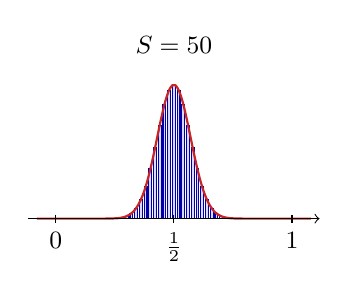
\begin{tikzpicture}[font=\small]
  \draw[fill=blue!15, draw=blue!65!black] (0.762,0) rectangle (0.798,0.005);
  \draw[fill=blue!15, draw=blue!65!black] (0.822,0) rectangle (0.858,0.013);
  \draw[fill=blue!15, draw=blue!65!black] (0.882,0) rectangle (0.918,0.030);
  \draw[fill=blue!15, draw=blue!65!black] (0.942,0) rectangle (0.978,0.066);
  \draw[fill=blue!15, draw=blue!65!black] (1.002,0) rectangle (1.038,0.132);
  \draw[fill=blue!15, draw=blue!65!black] (1.062,0) rectangle (1.098,0.242);
  \draw[fill=blue!15, draw=blue!65!black] (1.122,0) rectangle (1.158,0.407);
  \draw[fill=blue!15, draw=blue!65!black] (1.182,0) rectangle (1.218,0.631);
  \draw[fill=blue!15, draw=blue!65!black] (1.242,0) rectangle (1.278,0.901);
  \draw[fill=blue!15, draw=blue!65!black] (1.302,0) rectangle (1.338,1.188);
  \draw[fill=blue!15, draw=blue!65!black] (1.362,0) rectangle (1.398,1.446);
  \draw[fill=blue!15, draw=blue!65!black] (1.422,0) rectangle (1.458,1.626);
  \draw[fill=blue!15, draw=blue!65!black] (1.482,0) rectangle (1.518,1.692);
  \draw[fill=blue!15, draw=blue!65!black] (1.542,0) rectangle (1.578,1.626);
  \draw[fill=blue!15, draw=blue!65!black] (1.602,0) rectangle (1.638,1.446);
  \draw[fill=blue!15, draw=blue!65!black] (1.662,0) rectangle (1.698,1.188);
  \draw[fill=blue!15, draw=blue!65!black] (1.722,0) rectangle (1.758,0.901);
  \draw[fill=blue!15, draw=blue!65!black] (1.782,0) rectangle (1.818,0.631);
  \draw[fill=blue!15, draw=blue!65!black] (1.842,0) rectangle (1.878,0.407);
  \draw[fill=blue!15, draw=blue!65!black] (1.902,0) rectangle (1.938,0.242);
  \draw[fill=blue!15, draw=blue!65!black] (1.962,0) rectangle (1.998,0.132);
  \draw[fill=blue!15, draw=blue!65!black] (2.022,0) rectangle (2.058,0.066);
  \draw[fill=blue!15, draw=blue!65!black] (2.082,0) rectangle (2.118,0.030);
  \draw[fill=blue!15, draw=blue!65!black] (2.142,0) rectangle (2.178,0.013);
  \draw[fill=blue!15, draw=blue!65!black] (2.202,0) rectangle (2.238,0.005);
  \draw[redink, thick] plot[smooth] coordinates {(-0.240,0.000) (-0.201,0.000) (-0.162,0.000) (-0.123,0.000) (-0.084,0.000) (-0.044,0.000) (-0.005,0.000) (0.034,0.000) (0.073,0.000) (0.112,0.000) (0.151,0.000) (0.190,0.000) (0.229,0.000) (0.268,0.000) (0.307,0.000) (0.347,0.000) (0.386,0.000) (0.425,0.000) (0.464,0.000) (0.503,0.000) (0.542,0.000) (0.581,0.000) (0.620,0.000) (0.659,0.001) (0.698,0.001) (0.738,0.003) (0.777,0.005) (0.816,0.009) (0.855,0.017) (0.894,0.029) (0.933,0.048) (0.972,0.077) (1.011,0.120) (1.050,0.180) (1.089,0.261) (1.129,0.367) (1.168,0.498) (1.207,0.654) (1.246,0.829) (1.285,1.017) (1.324,1.205) (1.363,1.381) (1.402,1.529) (1.441,1.636) (1.480,1.693) (1.520,1.693) (1.559,1.636) (1.598,1.529) (1.637,1.381) (1.676,1.205) (1.715,1.017) (1.754,0.829) (1.793,0.654) (1.832,0.498) (1.871,0.367) (1.911,0.261) (1.950,0.180) (1.989,0.120) (2.028,0.077) (2.067,0.048) (2.106,0.029) (2.145,0.017) (2.184,0.009) (2.223,0.005) (2.262,0.003) (2.302,0.001) (2.341,0.001) (2.380,0.000) (2.419,0.000) (2.458,0.000) (2.497,0.000) (2.536,0.000) (2.575,0.000) (2.614,0.000) (2.653,0.000) (2.693,0.000) (2.732,0.000) (2.771,0.000) (2.810,0.000) (2.849,0.000) (2.888,0.000) (2.927,0.000) (2.966,0.000) (3.005,0.000) (3.044,0.000) (3.084,0.000) (3.123,0.000) (3.162,0.000) (3.201,0.000) (3.240,0.000)};
  \draw[->] (-0.35,0) -- (3.35,0);
  \foreach \v/\lab in {0/0, 1.5/\tfrac12, 3.0/1}
    { \draw (\v,0.05) -- (\v,-0.05) node[below] {$\lab$}; }
  \node at (1.5,2.2) {$S = 50$};
\end{tikzpicture}
\end{center}
\vspace{2pt}

\begin{center}
{\small bars: \ $\mathbb{P}\big(\tfrac{1}{S}\tilde\chi_S = \cdot\,\big)$ \qquad
{\color{redink}curve: \ $\mathcal{N}\big(\tfrac12, \tfrac{1}{4S}\big)$}}
\end{center}
\vspace{12pt}

\quad $S = 100$: \qquad $\dfrac{\sigma}{\sqrt{S}} = \dfrac{1/2}{10} = 0.05$, \qquad
$\mathbb{P}\big(0.40 \le \tfrac{1}{S}\tilde\chi_S \le 0.60\big) \approx 0.95$
\quad {\color{redink}$\big(\mu \pm 2\,\sigma/\sqrt{S}\big)$}
\vspace{12pt}

\begin{center}
\begin{tabular}{@{}r|ccc@{}}
 $S$ & $1$ & $100$ & $10{,}000$ \\ \hline
 \rule{0pt}{2.6ex}$\sigma/\sqrt{S}$ & $0.5$ & $0.05$ & $0.005$ \\
\end{tabular}
\end{center}
\vspace{6pt}

\quad {\color{redink}$10\times$ more precise \ needs \ $100\times$ more samples}
\vspace{8pt}

\quad {\color{redink}$S = 1$: \ one decision, made once --- nothing averages out; \ the spread stays $\sigma$}
\end{board}

\newpage
% ---------------------------------------------------------------- 2
\beat{2}{Duality theory}
\begin{board}
in this course, we focus on \textbf{convex} functions.
\vspace{10pt}

\textbf{Primal Problem}
\vspace{2pt}

\begin{center}
$\begin{aligned}
  \inf\quad & f_0(x) \\
  \text{s.t.}\quad & x \in \mathbb{R}^N \\
                   & f_i(x) \le 0 \qquad \forall i \in [I]
\end{aligned}$
\hspace{4.5cm} $(P)$
\end{center}
\vspace{10pt}

\textbf{Dual Problem}
\vspace{2pt}

\begin{center}
$\begin{aligned}
  \sup_{\theta}\ \inf_{x \in \mathbb{R}^N}\quad & f_0(x) + \sum_{i \in [I]} \theta_i f_i(x) \\
  \text{s.t.}\quad & \theta \in \mathbb{R}^I \\
                   & \theta \ge 0
\end{aligned}$
\hspace{4.0cm} $(D)$
\end{center}
\vspace{12pt}

\begin{center}
{\setlength{\arrayrulewidth}{1pt}
\arrayrulecolor{boxink}
\begin{tabular}{|@{\;}c@{\;\;}l@{\;}|}
\hline
\rule{0pt}{4.6em}
 & \color{redink}$\begin{aligned}
      \inf\quad & f_0(x) \\
      \text{s.t.}\quad & x \in \mathbb{R}^N \\
                       & f_i(x) \le 0 \qquad \forall i \in [I]
   \end{aligned}$ \\[1.4em]
\hline
\rule{0pt}{3.6em}
\color{redink}$=$ &
 \color{redink}$\displaystyle \inf_{x \in \mathbb{R}^N}\ f_0(x)
   \;+\; \underbrace{\ \sup_{\theta \in \mathbb{R}^I_+}\ \sum_{i \in [I]} \theta_i f_i(x)\ }_{\textstyle \color{purpink}\le\, 0}$ \\[2.6em]
\hline
\end{tabular}}
\end{center}
\vspace{4pt}

\hspace{3.0cm}{\color{purpink}if \ $f_i(x) \le 0 \ \ \forall i$, \quad then \quad $= 0$}
\vspace{3pt}

\hspace{3.0cm}{\color{purpink}if \ $\exists\, i : f_i(x) > 0$, \quad then \quad $= +\infty$}
\vspace{8pt}

{\color{redink}$\displaystyle \ \ \ge\ \ \sup_{\theta \in \mathbb{R}^I_+}\ \inf_{x \in \mathbb{R}^N}\ f_0(x)
  + \sum_{i \in [I]} \theta_i f_i(x)$}
\vspace{14pt}

\textbf{Properties:}
\vspace{4pt}

\quad --- \textbf{weak duality} \qquad $\inf\,(P) \ \ge\ \sup\,(D)$ \qquad always holds.
\vspace{6pt}

\quad --- \textbf{strong duality:} \qquad $\inf\,(P) \ =\ \sup\,(D)$ \ holds
\vspace{3pt}

\qquad\quad when the problem $(P)$ is convex and the \underline{Slater's condition} holds
\vspace{3pt}

\hspace{4.2cm}{\color{redink}$\exists\, x \in \mathbb{R}^N$, \ s.t. \ $f_i(x) < 0 \quad \forall i \in [I]$}
\newpage

\begin{center}
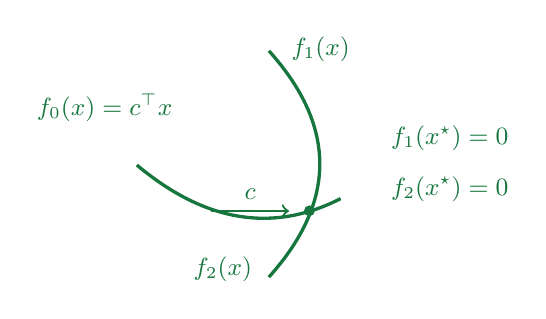
\begin{tikzpicture}[scale=1.15, font=\small]
  \draw[grnink, very thick] plot[domain=-1.25:1.25, samples=60]
        ({0.62 - 0.36*\x*\x}, {\x});
  \draw[grnink, very thick] plot[domain=-1.40:0.85, samples=60]
        ({\x}, {-0.60 + 0.30*\x*\x});
  \fill[grnink] (0.505,-0.518) circle (1.7pt);
  \draw[grnink, ->, thick] (-0.58,-0.52) -- (0.28,-0.52);
  \node[grnink, above] at (-0.15,-0.50) {$c$};
  \node[grnink, anchor=east] at (-0.90,0.62) {$f_0(x) = c^{\top}x$};
  \node[grnink, anchor=south west] at (0.20,1.02) {$f_1(x)$};
  \node[grnink, below] at (-0.45,-0.92) {$f_2(x)$};
  \node[grnink, anchor=west] at (1.30,0.28) {$f_1(x^\star) = 0$};
  \node[grnink, anchor=west] at (1.30,-0.28) {$f_2(x^\star) = 0$};
\end{tikzpicture}
\end{center}
\vspace{6pt}

{\color{redink}\textbf{In this course, we assume that strong duality holds for convex problem!!}}
\end{board}

% ---------------------------------------------------------------- 3
\beat{3}{Example: linear program}
\begin{board}
\textbf{Primal LP:}
\vspace{2pt}

\begin{center}
$\begin{aligned}
  \inf\quad & c^{\top}x \\
  \text{s.t.}\quad & x \in \mathbb{R}^N \\
                   & Ax \le b
\end{aligned}$
\hspace{1.8cm}
$\begin{aligned}
  & f_0(x) = c^{\top}x \\
  & f_i(x) = a_i^{\top}x - b_i \qquad \forall i \in [I]
\end{aligned}$
\end{center}
\vspace{4pt}

\hspace{6.6cm}{\color{redink}$f_i(x) \le 0$}
\vspace{3pt}

\hspace{6.1cm}{\color{redink}$\iff\ a_i^{\top}x - b_i \le 0$}
\vspace{3pt}

\hspace{6.1cm}{\color{redink}$\iff\ a_i^{\top}x \le b_i$}
\vspace{14pt}

\textbf{Dual LP:}
\vspace{4pt}

\quad $\displaystyle \sup_{\theta \in \mathbb{R}^I_+}\ \inf_{x \in \mathbb{R}^N}\
  c^{\top}x + \sum_{i \in [I]} \theta_i \big(a_i^{\top}x - b_i\big)$
\vspace{8pt}

$\displaystyle =\ \sup_{\theta \in \mathbb{R}^I_+}\ \inf_{x \in \mathbb{R}^N}\
  c^{\top}x + \sum_{i \in [I]} \theta_i a_i^{\top}x - \sum_{i \in [I]} \theta_i b_i$
\vspace{8pt}

$\displaystyle =\ \sup_{\theta \in \mathbb{R}^I_+}\ -\sum_{i \in [I]} \theta_i b_i
  \ +\ \inf_{x \in \mathbb{R}^N}\ \underbrace{\Big(c + \sum_{i \in [I]} \theta_i a_i\Big)^{\!\top} x}_{}$
\vspace{2pt}

\hspace{5.1cm}{\color{redink}$= \begin{cases}
   0 & \text{if } \ c + \sum_{i \in [I]} \theta_i a_i = 0 \\[4pt]
   -\infty & \text{if } \ \text{otherwise.}
 \end{cases}$}
\vspace{10pt}

$\begin{aligned}
  =\ \sup\quad & -b^{\top}\theta \\
  \text{s.t.}\quad & \theta \in \mathbb{R}^I_+ \\
                   & A^{\top}\theta = -c
\end{aligned}$
\vspace{16pt}

\underline{\textbf{LP strong duality}} : \ if there exists \ $x \in \mathbb{R}^N : Ax \le b$
\vspace{4pt}

\hspace{4.0cm} or \quad $\theta \in \mathbb{R}^I : A^{\top}\theta = -c, \ \ \theta \ge 0$
\vspace{6pt}

\hspace{2.7cm} then strong duality holds
\end{board}

\newpage
% ---------------------------------------------------------------- 4
\beat{4}{Conic programming}
\begin{board}
a conic program is a convex optimization problem.
\vspace{5pt}

\quad --- a \textbf{linear} objective function.
\vspace{4pt}

\quad --- a feasible set defines through the intersection of \underline{halfspaces}
\ {\color{redink}$Ax \le b$} \ or a proper cone.
\vspace{14pt}

\textbf{Def} (\emph{cone}) \quad a set $C$ is a cone if \ $\forall x \in C$, \ we have
$\lambda x \in C \quad \forall \lambda \ge 0$
\vspace{8pt}

\begin{center}
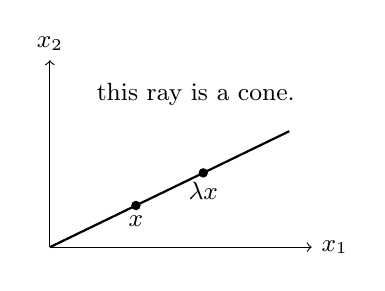
\begin{tikzpicture}[scale=0.95, font=\small]
  \draw[->] (0,0) -- (3.5,0) node[right] {$x_1$};
  \draw[->] (0,0) -- (0,2.5) node[above] {$x_2$};
  \draw[thick] (0,0) -- (3.2,1.55);
  \fill (1.15,0.557) circle (1.8pt) node[below] {$x$};
  \fill (2.05,0.993) circle (1.8pt) node[below] {$\lambda x$};
  \node at (1.95,2.05) {this ray is a cone.};
\end{tikzpicture}
\hspace{10mm}
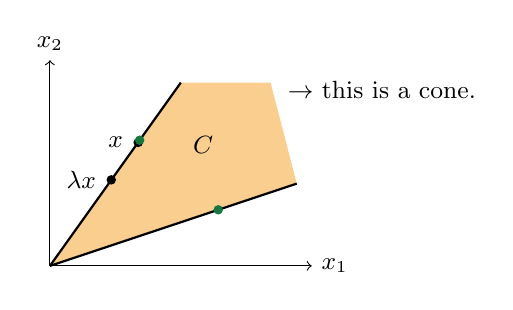
\begin{tikzpicture}[scale=0.95, font=\small]
  \fill[sandink] (0,0) -- (1.75,2.45) -- (2.95,2.45) -- (3.3,1.1) -- cycle;
  \draw[->] (0,0) -- (3.5,0) node[right] {$x_1$};
  \draw[->] (0,0) -- (0,2.75) node[above] {$x_2$};
  \draw[thick] (0,0) -- (1.75,2.45);
  \draw[thick] (0,0) -- (3.3,1.1);
  \fill (1.18,1.65) circle (1.8pt) node[anchor=east, xshift=-2pt] {$x$};
  \fill (0.82,1.15) circle (1.8pt) node[anchor=east, xshift=-2pt] {$\lambda x$};
  \fill[grnink] (1.20,1.68) circle (1.8pt);
  \fill[grnink] (2.25,0.75) circle (1.8pt);
  \node at (2.05,1.62) {$C$};
  \node[anchor=west] at (3.05,2.35) {$\rightarrow$ this is a cone.};
\end{tikzpicture}
\end{center}
\vspace{12pt}

\textbf{Def} (\emph{proper cone}) \hspace{2.2cm}
{\color{magink}$\mathbb{R}^N$ is a cone but not pointed.}
\vspace{5pt}

\quad $C$ is a proper cone if it's \textbf{convex}, \textbf{closed}, \underline{\textbf{pointed}}
\vspace{4pt}

\hspace{4.7cm}{\color{redink}if \ $x, -x \in C$ \ then \ $x = 0$.}
\vspace{14pt}

\textbf{Generic conic program:}
\vspace{2pt}

\begin{center}
$\begin{aligned}
  \inf\quad & c^{\top}x \\
  \text{s.t.}\quad & x \in \mathbb{R}^N \\
                   & Ax \coneleq b
\end{aligned}$
\hspace{1.4cm}{\color{redink}$\iff\ \ b - Ax \in C$}
\end{center}
\vspace{14pt}

\textbf{Example:}
\vspace{8pt}

\quad 1) \textbf{Linear program:} \quad $C = \mathbb{R}^K_+$
\vspace{6pt}

\begin{center}
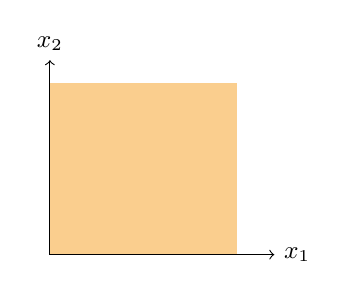
\begin{tikzpicture}[scale=0.95, font=\small]
  \fill[sandink] (0,0) rectangle (2.5,2.3);
  \draw[->] (0,0) -- (3.0,0) node[right] {$x_1$};
  \draw[->] (0,0) -- (0,2.6) node[above] {$x_2$};
\end{tikzpicture}
\hspace{16mm}
\raisebox{13mm}{$\begin{aligned}
  & b - Ax \in \mathbb{R}^K_+ \\[8pt]
  \iff\ & b - Ax \ge 0 \ \iff\ Ax \le b
\end{aligned}$}
\end{center}
\vspace{14pt}

\quad 2) \textbf{Semidefinite program:} \quad $C = \mathbb{S}^K_+$
\vspace{8pt}

\hspace{0.7cm}{\color{redink}$\mathbb{S}^K$ : set of symmetric matrices in $\mathbb{R}^{K \times K}$ \quad $(A^{\top} = A)$}
\vspace{5pt}

\hspace{0.7cm}{\color{redink}$\mathbb{S}^K_+$ : set of positive semidefinite (symmetric) matrices in $\mathbb{R}^{K \times K}$}
\vspace{4pt}

\hspace{2.0cm}{\color{redink}$A \in \mathbb{S}^K_+$ \ if \ $z^{\top}Az \ge 0 \qquad \forall z \in \mathbb{R}^K$}
\vspace{10pt}

\qquad \textbf{Generic semidefinite program:}
\vspace{2pt}

\begin{center}
$\begin{aligned}
  \inf\quad & c^{\top}x \\
  \text{s.t.}\quad & x \in \mathbb{R}^N \\
                   & A_1 x_1 + A_2 x_2 + \cdots + A_N x_N
                     \mathrel{\preceq_{\textcolor{redink}{\mathbb{S}^K_+}}} B
\end{aligned}$
\hspace{0.8cm}{\color{redink}\small $\rightarrow$ usually ignored}
\end{center}
\newpage

\quad 3) \textbf{Second-order cone:} \quad
$C = \big\{ (x,t) \in \mathbb{R}^N \times \mathbb{R} \;:\; \|x\|_2 \le t \big\}$
\qquad ``ice-cream'' cone
\vspace{6pt}

\begin{center}
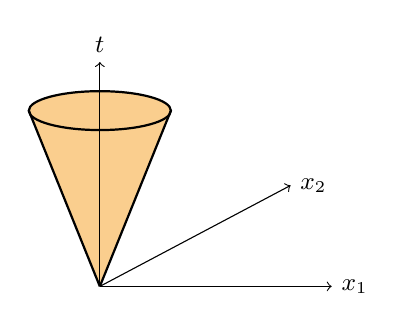
\begin{tikzpicture}[scale=0.95, font=\small]
  \fill[sandink] (0,0) -- (-0.95,2.35) -- (0.95,2.35) -- cycle;
  \fill[sandink] (0,2.35) ellipse (0.95 and 0.26);
  \draw[->] (0,0) -- (0,3.0) node[above] {$t$};
  \draw[->] (0,0) -- (2.55,1.35) node[right] {$x_2$};
  \draw[->] (0,0) -- (3.1,0) node[right] {$x_1$};
  \draw[thick] (0,2.35) ellipse (0.95 and 0.26);
  \draw[thick] (0,0) -- (-0.95,2.35);
  \draw[thick] (0,0) -- (0.95,2.35);
\end{tikzpicture}
\hspace{18mm}
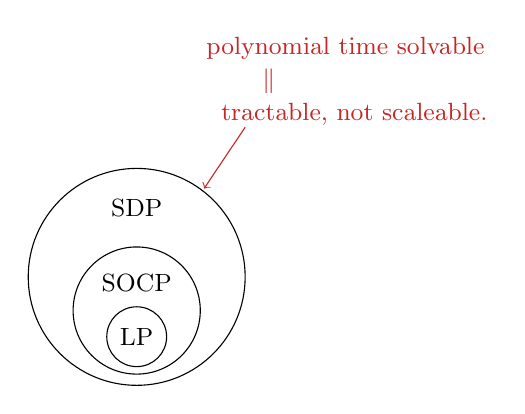
\begin{tikzpicture}[scale=0.95, font=\small]
  \draw (0,0) circle (1.45);
  \draw (0,-0.45) circle (0.85);
  \draw (0,-0.80) circle (0.40);
  \node at (0,-0.80) {LP};
  \node at (0,-0.08) {SOCP};
  \node at (0,0.92) {SDP};
  \draw[redink, ->] (1.45,2.00) -- (0.90,1.18);
  \node[redink, anchor=west] at (1.00,2.18) {tractable, not scaleable.};
  \node[redink, anchor=west] at (1.55,2.62) {$\parallel$};
  \node[redink, anchor=west] at (0.80,3.06) {polynomial time solvable};
\end{tikzpicture}
\end{center}
\end{board}

% ---------------------------------------------------------------- 5
\beat{5}{Conic programming duality}
\begin{board}
\textbf{Def} (\emph{dual cone})
\vspace{4pt}

\quad $C^* = \big\{\, y \in \mathbb{R}^K \;:\; \langle y, x \rangle \ge 0 \quad \forall x \in C \,\big\}$
\vspace{14pt}

\textbf{Self dual cones} \ $(C = C^*)$
\vspace{5pt}

\quad --- $C = \hl{\mathbb{R}^K_+}$
\vspace{5pt}

\quad --- $C = \hl{\mathbb{S}^K_+}$
\vspace{5pt}

\quad --- $C = $ \colorbox{hlyel}{second-order cone}
\vspace{16pt}

\textbf{Primal conic program:}
\vspace{2pt}

\begin{center}
$\begin{aligned}
  \inf\quad & c^{\top}x \\
  \text{s.t.}\quad & x \in \mathbb{R}^N \\
                   & Ax \coneleq b
\end{aligned}$
\end{center}
\vspace{12pt}

\textbf{Dual conic program:}
\vspace{2pt}

\begin{center}
$\begin{aligned}
  \sup\quad & -\theta^{\top}b \\
  \text{s.t.}\quad & \theta \in \hl{C^*} \\
                   & A^{\top}\theta = -c
\end{aligned}$
\end{center}
\end{board}

\end{document}
